\documentclass{beamer}

%\usepackage{subfigure}
\usepackage{graphicx}
\usepackage{sidecap}
\usepackage{caption}
\usepackage{subcaption}
\captionsetup{compatibility=false}
\usepackage{appendixnumberbeamer}
\usepackage{amsmath}
% --
\usepackage{multirow}
\usepackage{xcolor}
\usepackage{setspace}
\usepackage{hyperref}
\usepackage{anyfontsize}

\setbeamertemplate{footline}

\newenvironment{itemise} {\begin{itemize} \setlength{\itemsep}{0.2cm}} {\end{itemize}}
\usepackage[labelformat=empty]{caption}
\setbeamertemplate{sections/subsections in toc}[square]

%% COLORS
\definecolor{Gray}{gray}{0.9}
\definecolor{dblue}{rgb}{0.132,0.1,0.27}
\definecolor{mint}{cmyk}{1.0, 0.2, 0.6, 0.05}
\definecolor{ant}{cmyk}{0.5, 0.1, 0.0, 0.45}
\definecolor{lgray}{cmyk}{0.12, 0.0, 0.0, 0.17}
\definecolor{lred}{cmyk}{0.0, 0.9, 0.7, 0.0}


\usepackage{etoolbox}% http://ctan.org/pkg/etoolbox 
\usepackage{booktabs}

\newenvironment{literatur}{%
  \parskip2pt \parindent0pt \raggedright
  \def\lititem{\hangindent=0.5cm \hangafter1}}{%
  \par\ignorespaces}

\newcommand{\tb}[1]{{\color{blue}{\textbf{#1}}}}
\newcommand{\tm}[1]{{\color{mint}{\textbf{#1}}}}
\newcommand{\tr}[1]{{\color{red}{\textbf{#1}}}}
% Ilya: packages

\usepackage{tikz}
\usepackage{lmodern}
\usepackage{enumitem}

% Ilya: my commands

\newenvironment{mytemize}
{\vfill\itemize[nolistsep,itemsep=\fill,label=\color{blue}{$\triangleright$}]}
  {\enditemize}


\newenvironment{mynumerate}
{\vfill\enumerate[nolistsep,itemsep=\fill,label=\arabic*.]}
  {\endenumerate}

\newcommand{\hitem}[1]{
  {\color{blue}{$\triangleright$}} 
  {#1} 
  {\hfill}
}

\setlist[itemize]{label= \color{blue}{$\triangleright$}}
\setlist[enumerate]{label = \arabic*.}

\newcommand{\rarr}{$\Rightarrow$\ }



%\href{<Ziel>}{<Eingefasster Text>} 

%\logo{\includegraphics[height=0.7cm]{BdFlogo.eps}\hspace{300pt}\vspace{-5pt}}
%\logo{\includegraphics[height=0.8cm]{BdFlogo.eps}}
%\logo{\pgfputat{\pgfxy(-6.2,-0.5)}{\pgfbox[center,base]{\includegraphics[height=0.8cm]{BdFlogo.eps}}}}

%------------------------------------------------------------------------------------
% TITLE
%------------------------------------------------------------------------------------
\title[PSME]{Macroeconomics\\ Lecture 7 -- RBC: additional topics} 
\author[I. Eryzhenskiy]{Ilya Eryzhenskiy}
\institute[BdF]{PSME Panth\'{e}on-Sorbonne Master in Economics}
\date[PSME macro]{Fall 2022}

%---BEGIN------------------------------------------------------------------------------
\begin{document}

\begin{frame}
  \maketitle
\end{frame}

\begin{frame}{Overview}
  \tableofcontents
\end{frame}

\section{Equilibrium optimality}
\begin{frame}{Social planner's problem}

\begin{mytemize}
\item The Social Planner
\begin{mytemize}
\item A fictional entity used to  to talk about optimal outcomes
\item Is \tb{benevolent} \rarr maximizes utility of representative household
\item Instead of optimizing w.r.t. prices, can reallocate goods between agents with no transaction cost 
  \rarr prices omitted from optimality analysis
\end{mytemize}
\item  The Social planner problem $\leftrightarrow$ finding optimal allocations:
\begin{mytemize}
\item Maximize a welfare criterion (benevolent \rarr HH utility)
\item ...subject to resource constraints -- physical constraints of economy
\end{mytemize}
\end{mytemize}


\end{frame}
%---FRAME------------------------------------------------------------------------------
\begin{frame}{Social Planner Optimization}


\begin{align*}
\max_{\left\{ C_t, L_t, K_{t+1} \right\}} E_0 \sum_{t=0}^{\infty} \beta^t  u(C_t,1-L_t)
\end{align*}
s.t. a \emph{sequence} of \tb{resource constraints}:
\begin{align*}
C_t + K_{t+1}-(1-\delta)K_t = Z_t f(K_t,L_t) \quad \text{for each } t=0,1,2,...
\end{align*}
FOCs of the Lagrangian with multipliers $\{\lambda_t\}$:
\begin{align*}
&(1) \quad \frac{\partial \mathcal{L}}{C_t} &= 0: \ \   & u'_c(C_t,1-L_t)-\lambda_t = 0\\
&(2) \quad \frac{\partial \mathcal{L}}{L_t} &= 0: \ \   &-u'_{1-L}(C_t,1-L_t)+\lambda_t Z_t f'_L(K_t,L_t)=0\\
&(3) \quad \frac{\partial \mathcal{L}}{K_{t+1}} &= 0: \ \   &-\lambda_t  +\beta E_t[\lambda_{t+1}(1+Z_{t+1}f'_K(K_{t+1},L_{t+1})-\delta)]=0 \\
\end{align*}

\end{frame}
%---FRAME------------------------------------------------------------------------------
\begin{frame}{Optimal allocations}

  \tb{Efficient allocation} is a sequence $\{C_t, L_{t}, K_{t+1}\}_{t=0}^\infty$, that, given $K_0, Z_0$ and the exogenous stochastic process $\ln Z_t = \rho \ln Z_{t-1} + \epsilon_t$, solves the social planner's optimization problem, i.e. satisfies the FOCs:
\begin{align*}
1 =& E_t \left[ \left( \frac{\beta \lambda_{t+1}}{\lambda_t}\right)(1+Z_{t+1} f'_K(K_{t+1},L_{t+1})-\delta)\right] \nonumber\\
\frac{u'_{1-L}(C_t,1-L_t)}{u'_c(C_t,1-L_t)}=& Z_t f'_L(K_t,L_t) \nonumber\\
C_t+K_{t+1}-(1-\delta)K_t=& Z_t f(K_t,L_t) \nonumber
\end{align*}
...which also gave the \tr{equilibrium}! \rarr \tb{equilibrium is optimal} \\
\vfill
$\rightarrow$ \tm{First Welfare Theorem} (\textit{see Microeconomics}) in a production economy with 1 agent and an $\infty$ of goods $\{C_t, 1-L_{t}\}_{t=0}^\infty$.
\vfill
Note that the social planner does not need prices to achieve the same allocation.
\end{frame}

\section{Compact specification of model}
\begin{frame}{Compact specification of model}
  Specification of RBC used most often has the household owning the capital stock directly, without the wealth variable $\Omega$.
  \vfill
  Investment variable can be substituted from the resource constraint, the HH chooses $K_{t+1}$ directly (like the Social planner).
  \vfill 
  Firms then \textbf{rent} the capital from HH, paying a \tb{rental rate of capital} $R_t$.
  \vfill
  Additionally, existence of \tb{bond market} assumed, where households make savings by holding bonds of real value $B_{t+t}$ in period $t$. Optimizing w.r.t. $B_{t+1}$ gives the Euler equation. Without the government and with identical households $B_t = 0 \ \ \forall t$ in equilibrium.
\end{frame}

\begin{frame}{Compact specification of model}
  \tm{Representative household}: 
\begin{align*}
  \max _{C_{t}, L_{t}, I_t, B_{t+1}} &E_{0} \sum_{t=0}^{\infty} \beta^{t}(C_{t}, 1-L_{t}) \\
\text { s.t. } \quad
C_{t}+I_t+B_{t+1} &=  w_{t} L_{t}+R_{t} K_{t}+\Pi_{t}+(1+r_{t}) B_{t} \\
K_{t+1} &=  (1-\delta) K_{t}+I_t
\end{align*}
or, omitting $I_t$, household chooses $K_{t+1}$ directly: 
\begin{align*}
  \max _{C_{t}, L_{t}, K_{t+1}, B_{t+1}} &E_{0} \sum_{t=0}^{\infty} \beta^{t}(C_{t}, 1-L_{t}) \\
\text { s.t. } \ \
C_{t}+K_{t+1}+B_{t+1} &=  w_{t} L_{t}+R_{t} K_{t}+ (1-\delta)K_t +\Pi_{t}+(1+r_{t}) B_{t} 
\end{align*}
  \tm{Representative firm}: 
  $\max _{K_{t}, L_{t}} Z_t f(K_t, L_t) - w_t L_t -  R_t K_t$
\vfill
\tb{Bond market equilibrium}: $B_t = 0$ (since no government and identical households)
\vfill
\centering
\textbf{\textit{Home task: verify that equilibrium same as before}}

\end{frame}
%---FRAME------------------------------------------------------------------------------

\section{Capital adjustment cost}
\begin{frame}
\frametitle{Outline}
\tableofcontents[currentsection]
\end{frame}

\begin{frame}{Investment impulse responses: model vs. data}
  Investment is too ``jumpy'' in the baseline RBC w.r.t. data \\
  \vfill
  \rarr \tb{capital adjustment costs} introduced to model inertia.
  \begin{figure}
     \centering
     \begin{subfigure}[b]{0.46\textwidth}
         \centering
		 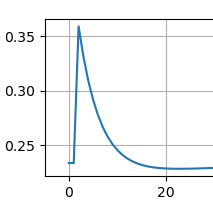
\includegraphics[width=\textwidth]{FIGURES/irf_i}
		 \caption{Model IRF}
     \end{subfigure}
      \hfill
     \begin{subfigure}[b]{0.52\textwidth}
         \centering
		 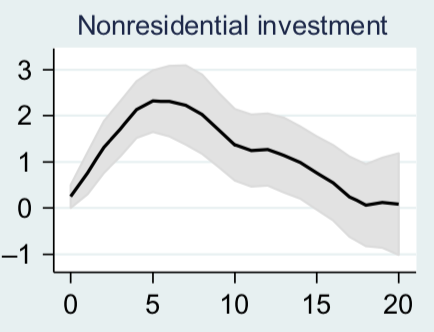
\includegraphics[width=\textwidth]{FIGURES/investment_VAR.png}
		 \caption{Empirical IRF (Ramey, 2016)}
     \end{subfigure}
	 \caption{Investment reaction to transitory productivity shock.}
\end{figure}
\end{frame}
\begin{frame}{Capital law of motion with adjustment costs}
  A new law of motion for capital: 
$$
K_{t+1}=I_{t}\textcolor{purple}{-\frac{\phi}{2}\left(\frac{I_{t}}{K_{t}}-\delta\right)^{2} K_{t}}+(1-\delta) K_{t}
$$
If $\phi>0$, then doing investment above or below steady state (in steady state $\frac{I_{ss}}{K_{ss}}=\delta$ ) results in a cost. Quadratic function: marginal cost increases as investment further from s.s. 
\end{frame}

\begin{frame}{Household problem}
  New household problem (in a compact form):
  $$
\begin{gathered}
\max _{C_{t}, I_{t}, L_{t}, K_{t+1}, B_{t+1}} E_{0} \sum_{t=0}^{\infty} \beta^{t}\left(\ln C_{t}-\theta \frac{L_{t}^{1+\chi}}{1+\chi}\right) \\
\text { s.t. } \quad
C_{t}+I_{t}+B_{t+1} =  w_{t} L_{t}+R_{t} K_{t}+\Pi_{t}+\left(1+r_t\right) B_{t} \\
K_{t+1}=I_{t}\textcolor{purple}{-\frac{\phi}{2}\left(\frac{I_{t}}{K_{t}}-\delta\right)^{2} K_{t}}+(1-\delta) K_{t}
\end{gathered}
$$
\end{frame}

\begin{frame}{Household problem -- solution}
A Lagrangian with two constraints \rarr two multipliers, $\lambda$ and $\mu$:
\begin{align*}
\mathcal{L}=E_{0} \sum_{t=0}^{\infty} &\beta^{t}\{\ln C_{t}-\theta \frac{L_{t}^{1+\chi}}{1+\chi} \\
&+\lambda_{t}(w_{t} L_{t}+R_{t} K_{t}+\Pi_{t}+\left(1+r_t\right) B_{t}-C_{t}-I_{t}-B_{t+1}) \\
&+\mu_{t}(I_{t}\textcolor{purple}{-\frac{\phi}{2}(\frac{I_{t}}{K_{t}}-\delta)^{2} K_{t}}+(1-\delta) K_{t}-K_{t+1})\}
\end{align*}
\end{frame}

\begin{frame}{Household problem -- solution}
The first order conditions are:
\begin{align*}
\frac{\partial \mathcal{L}}{\partial C_{t}}=0 &\Leftrightarrow \frac{1}{C_{t}}=\lambda_{t} \\
\frac{\partial \mathcal{L}}{\partial L_{t}}=0 &\Leftrightarrow \theta L_{t}^{\chi}=\lambda_{t} w_{t} \\
\frac{\partial \mathcal{L}}{\partial I_{t}}=0 &\Leftrightarrow \lambda_{t}=\mu_{t}(1-\phi(\frac{I_{t}}{K_{t}}-\delta)) \\
\frac{\partial \mathcal{L}}{\partial K_{t+1}}=0 &\Leftrightarrow  \\ \mu_{t}=\beta E_{t}[&R_{t+1} \lambda_{t+1}-\mu_{t+1} \frac{\phi}{2}(\frac{I_{t+1}}{K_{t+1}}-\delta)^{2} \\
&+\mu_{t+1} \phi(\frac{I_{t+1}}{K_{t+1}}-\delta) \frac{I_{t+1}}{K_{t+1}}+\mu_{t+1}(1-\delta)] \\
\frac{\partial \mathcal{L}}{\partial B_{t+1}}=0 &\Leftrightarrow \lambda_{t}=\beta E_{t} \lambda_{t+1}\left(1+r_{t}\right)
\end{align*}

\end{frame}

\begin{frame}{Tobin's q is back}

  We define \tb{$q_{t} \equiv \frac{\mu_{t}}{\lambda_{t}}$} 
\begin{mytemize}
\item	$\mu_{t}$ -- marginal utility of additional capital installed
\item $\lambda_{t}$ -- marginal utility of consumption 
\item The ratio $q_t$ -- how much consumption you would give up to have some extra future capital
\item At the same time, \textbf{the price of capital good is 1}, same as consumption good
\item[\rarr] $q_t$ is theoretical \tb{Tobin's q} -- ratio of willingness-to-pay to price of physical capital goods
\end{mytemize}
\vfill
The FOC $\frac{\partial \mathcal{L}}{\partial I_{t}}=0$ can be re-written: 
$
q_{t}=\left(1-\phi\left(\frac{I_{t}}{K_{t}}-\delta\right)\right)^{-1} 
$ \\
\vfill
\rarr positive association between $I_t$ and $q_t$: $I(\underset{+}{q_t},\dots)$ \\
\vfill
  Main implication for equilibrium: additional \tb{inertia} in investment.
\end{frame}

\begin{frame}{Impulse responses with various capital adjustment costs}
  \vspace{-0.3cm}
  \begin{figure}[ht]
	\centering
	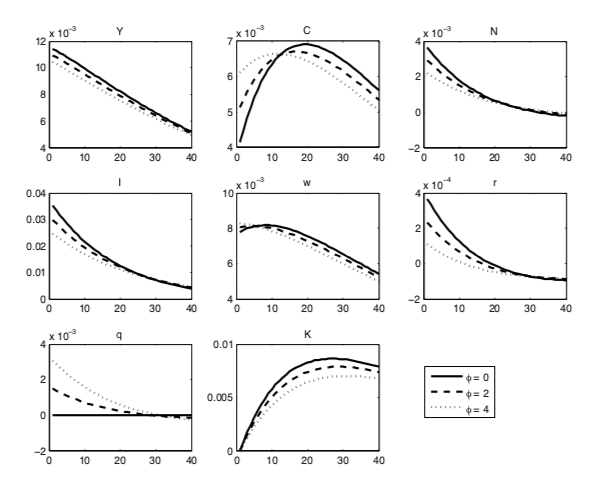
\includegraphics[width = 0.91\linewidth]{FIGURES/Adjust_cost_IRF_EricSims}
	\caption{Response to a transitory productivity shock under different values of $\phi$ -- capital adjustment cost magnitude}
  \end{figure}
\end{frame}

\begin{frame}{Alternative specifications}
  The form of adjustment cost is the simplest one; investment less reactive, but still not ``hump-shaped'' as in empirical IRF.

  Several other options exist:
  \begin{enumerate}
	\item Specified in HH budget constraint directly:
	  \begin{align*}
		C_t + I_t + B_{t+1} &= w_t L_t + R_t K_t \textcolor{purple}{- \frac{1}{2} \frac{I^2_t}{K_t}} \\
		\text{or} \quad	C_t + I_t + B_{t+1} &= w_t L_t + R_t K_t \textcolor{purple}{- \Phi(K_{t+1} - K_t)}, \ \text{with} \ \Phi', \Phi''>0 
	  \end{align*}
	\item Specified in law of motion of capital, but w.r.t. investment variable only -- \tb{investment adjustment cost}:
$$
K_{t+1}=\textcolor{purple}{\left[1-\frac{\phi}{2}\left(\frac{I_{t}}{I_{t-1}}-1\right)^2 \right]} I_{t}+(1-\delta) K_{t}
$$
Here, investment can be called both a \tm{state} and a \tm{control}. \\
\vfill
Investment adjustment cost is known to produce hump-shaped reactions of investment to productivity shocks.
  \end{enumerate}
\end{frame}


\begin{frame}{Investment adjustment cost -- impulse responses}
  \begin{figure}[ht]
	\centering
	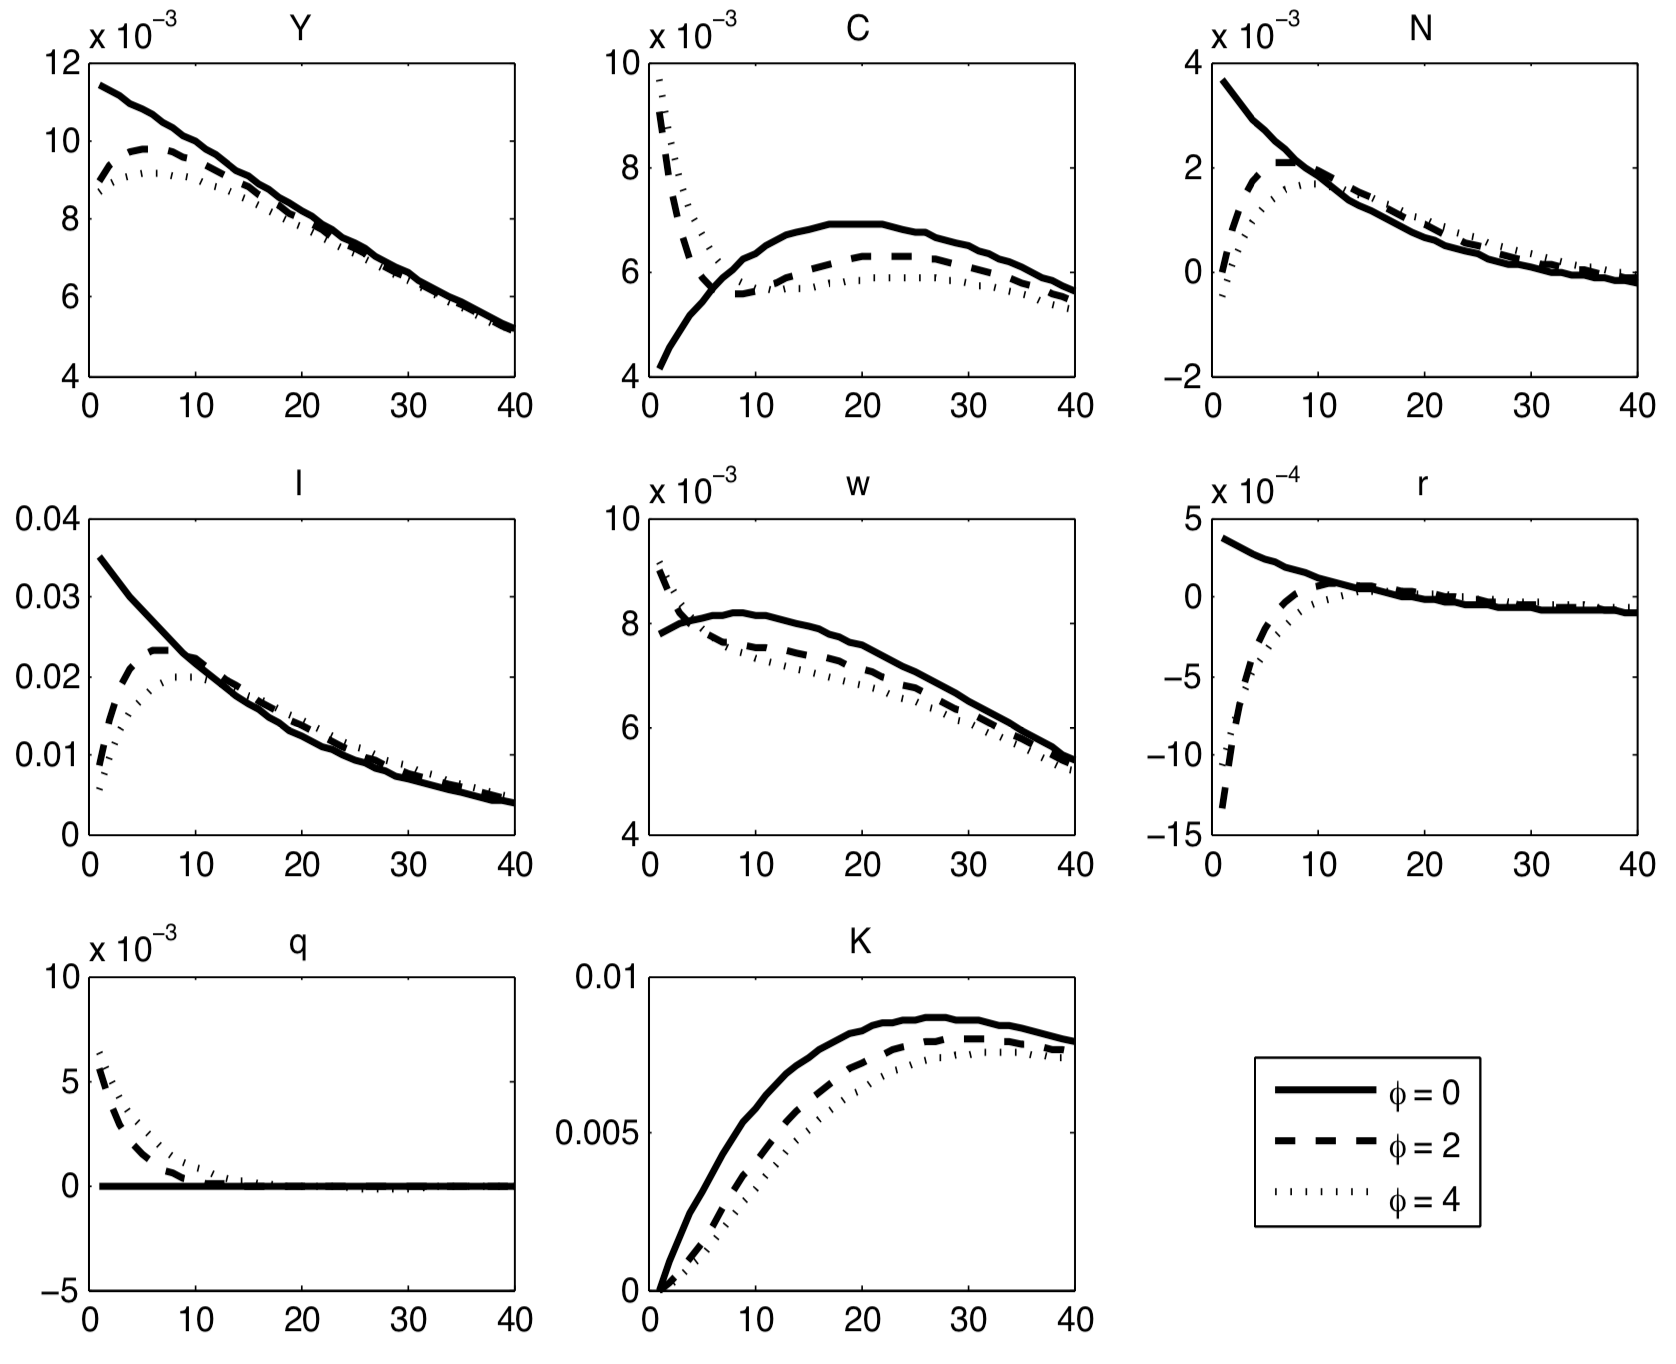
\includegraphics[width=0.95\textwidth]{FIGURES/inv_adj_cost_IRF_EricSims}
  \end{figure}
\end{frame}

\section{Models vs. data}
\begin{frame}
\frametitle{Outline}
\tableofcontents[currentsection]
\end{frame}

\begin{frame}{Model and data}
  We have seen how modelling assumptions changed to make an RBC model produce more realistic IRF. \\
\vfill
How to choose parameter values to make models as realistic as possible? Several approaches for RBC and, more generally, \tb{DSGE} (Dynamic Stochastic General Equilibrium) models:
\begin{mynumerate}
\item Use values that are established (consensual) in academic literature 
  \begin{mytemize}
  \item Example: $\alpha = 1/3$ (share of capital income in national income)
  \item must be careful about what is the ``literature'' we are looking at and what we call ``established''!
  \end{mytemize}
\item \tb{Calibration} $\rightarrow$ picking parameter values by hand to match some empirical \tb{target}, often about \textbf{steady state} 
  \begin{mytemize}
  \item Example: labor disutility coefficient chosen such that $L_{ss} = 1/3$, which comes (approximately) from U.S. statistics
  \item Related to General Method of Moments (GMM), which is an \tb{estimation} method (see below)
  \end{mytemize}
\end{mynumerate} 
\end{frame}
\begin{frame}{Model and data}
\begin{enumerate}
  \item[3.] \tb{Estimation} $\rightarrow$ automated \textbf{econometric} procedures; theory not covered in lectures, separate course needed. \\ 2 main classes of methods: 
  \begin{mytemize}
  \item \underline{Frequentist}: Rely on relationships between theoretical probabilities and empirical frequencies -- Law of Large Numbers \\ Use \tm{least squares} (less useful for macro than micro), \tm{GMM}, \tm{Maximum Likelihood}, \tm{Kalman filter}  
  \item \underline{Bayesian}: Rely on probabilities as \textbf{beliefs} of researcher; use data and Bayes rule to update prior beliefs (priors) to posterior beliefs (posteriors). \\ Use \tm{Maximum Likelihood}, \tm{Kalman filter}, \tm{Monte Carlo Markov Chains} methods 
  \end{mytemize}
\end{enumerate} 
  The TDs after the break will be focused on implementation of ML estimation.
\end{frame}
  
\begin{frame}
  \begin{figure}[ht]
	\centering
	
\includegraphics[width = 0.8\linewidth]{FIGURES/new_method_meme.png}
	\caption{A representation of how you will feel doing model estimation \\ (and it's \textit{normal})}
  \end{figure}
\end{frame}
\end{document}
